
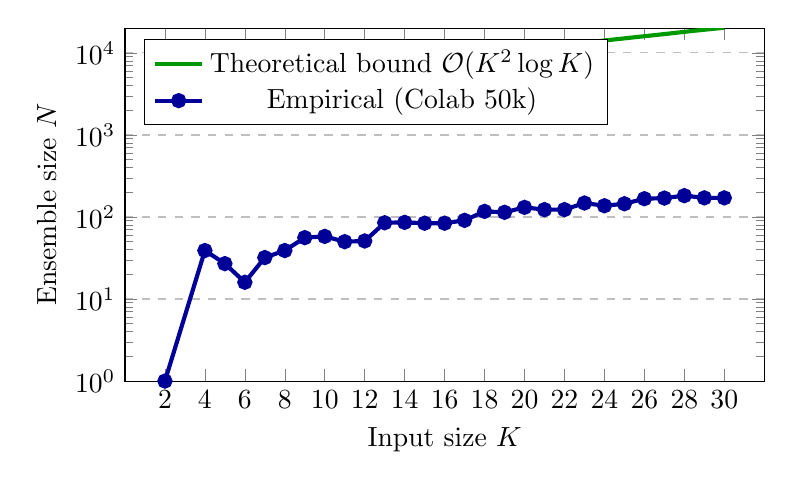
\begin{tikzpicture}
\begin{semilogyaxis}[
    width=0.8\textwidth,
    height=0.5\textwidth,
    title={}, % Title handled by caption in main.tex usually, but kept blank or specific
    xlabel={Input size $K$},
    ylabel={Ensemble size $N$},
    xmin=0, xmax=32,
    ymin=1, ymax=20000,
    xtick={2,4,6,8,10,12,14,16,18,20,22,24,26,28,30},
    % ytick={1,10,100,1000,10000},
    legend pos=north west,
    ymajorgrids=true,
    grid style=dashed,
]

% Theoretical Bound
\addplot[
    color=green!60!black,
    style=solid,
    line width=1.5pt,
]
coordinates {
    (2.0,5013.9) (3.5,5075.1) (4.9,5195.7) (6.4,5383.4) (7.9,5643.9) (9.4,5981.8) (10.8,6400.9) (12.3,6904.2) (13.8,7494.7) (15.3,8174.6) (16.7,8946.4) (18.2,9811.9) (19.7,10772.9) (21.2,11831.3) (22.6,12988.5) (24.1,14246.0) (25.6,15605.2) (27.1,17067.3) (28.5,18633.7) (30.0,20305.4) 
};
\addlegendentry{Theoretical bound $\mathcal{O}(K^2 \log K)$}

% Empirical Data
\addplot[
    color=blue!60!black,
    mark=*,
    style=solid,
    line width=1.5pt,
]
coordinates {
    (2,1) (3,0) (4,39) (5,27) (6,16) (7,32) (8,39) (9,56) (10,58) (11,50) (12,51) (13,85) (14,86) (15,84) (16,84) (17,91) (18,117) (19,114) (20,131) (21,123) (22,123) (23,148) (24,137) (25,145) (26,167) (27,170) (28,182) (29,171) (30,171) 
};
\addlegendentry{Empirical (Colab 50k)}

\end{semilogyaxis}
\end{tikzpicture}
